\documentclass[12pt]{article}
\usepackage{parskip}
\usepackage[paper=a4paper,left=25mm,right=25mm,top=30mm,bottom=30mm]{geometry}
\usepackage{fancyhdr}
\setlength{\headheight}{15pt}
\usepackage{ucs}
\usepackage[utf8x]{inputenc}
\usepackage[T1]{fontenc}
\usepackage{microtype}
\usepackage{amsmath,amssymb,amstext}
\usepackage{graphicx}
\usepackage{lmodern}

\PassOptionsToPackage{obeyspaces}{url}  % Url
\usepackage[hyphens]{xurl}
\usepackage{hyperref}
\usepackage[gen]{eurosym}  % Euro
%\usepackage[parmaite]{tengwarscript}  % Elvish
%\usepackage{pdfpages}  % Inclusion
%\usepackage{changepage}  % Signature

\pagestyle{fancy}
\fancyhf{}
\lhead{Lucas Aschenbach}
\chead{R-Projekt}
\rhead{Christoph Müßig}
\cfoot{\thepage}

\begin{document}
\begin{center}
    \begin{huge}
        R-Projekt
    \end{huge}
\end{center}

\section*{Einleitung}

Im November des vergangenen Jahres kündigt der Börsengigant ''S\&P Dow Jones Indices'' den ''S\&P 500 Twitter Sentiment Index'' an. Dabei handelt es sich um einen Aktienindex, der Wertpapiere nach ihrer aktuellen Popularität auf Twitter bewertet. Und es ist längst nicht der einzige Fall, in dem alteingessene Finanzmarkt-Akteure Interesse an Social Media Daten für Kursvorhersagen demonstrieren. Spätestens nach den Geschnissen um ''Game Stop'' im Januar 2021 wurde deutlich, welche Macht Kleininvestoren im Zeitalter der globalen Vernetzung entfalten können, wenn sie sich nur koordinieren.

Im hochvolatilen Crypto-Markt ist der Effekt noch ausgeprägter, im Kurs von ''Dogecoin'' hinterlässt jeder Tweet von Elon Musk deutliche Spuren. Wenn ein Coin große Popularität erreicht, ist aber eigentlich schon die größte Chance für Investoren vorbei. Man betrachte beispielshaft den historischen Wertkurs von ''Dogecoin'':

\begin{figure}[h]
    \centering
    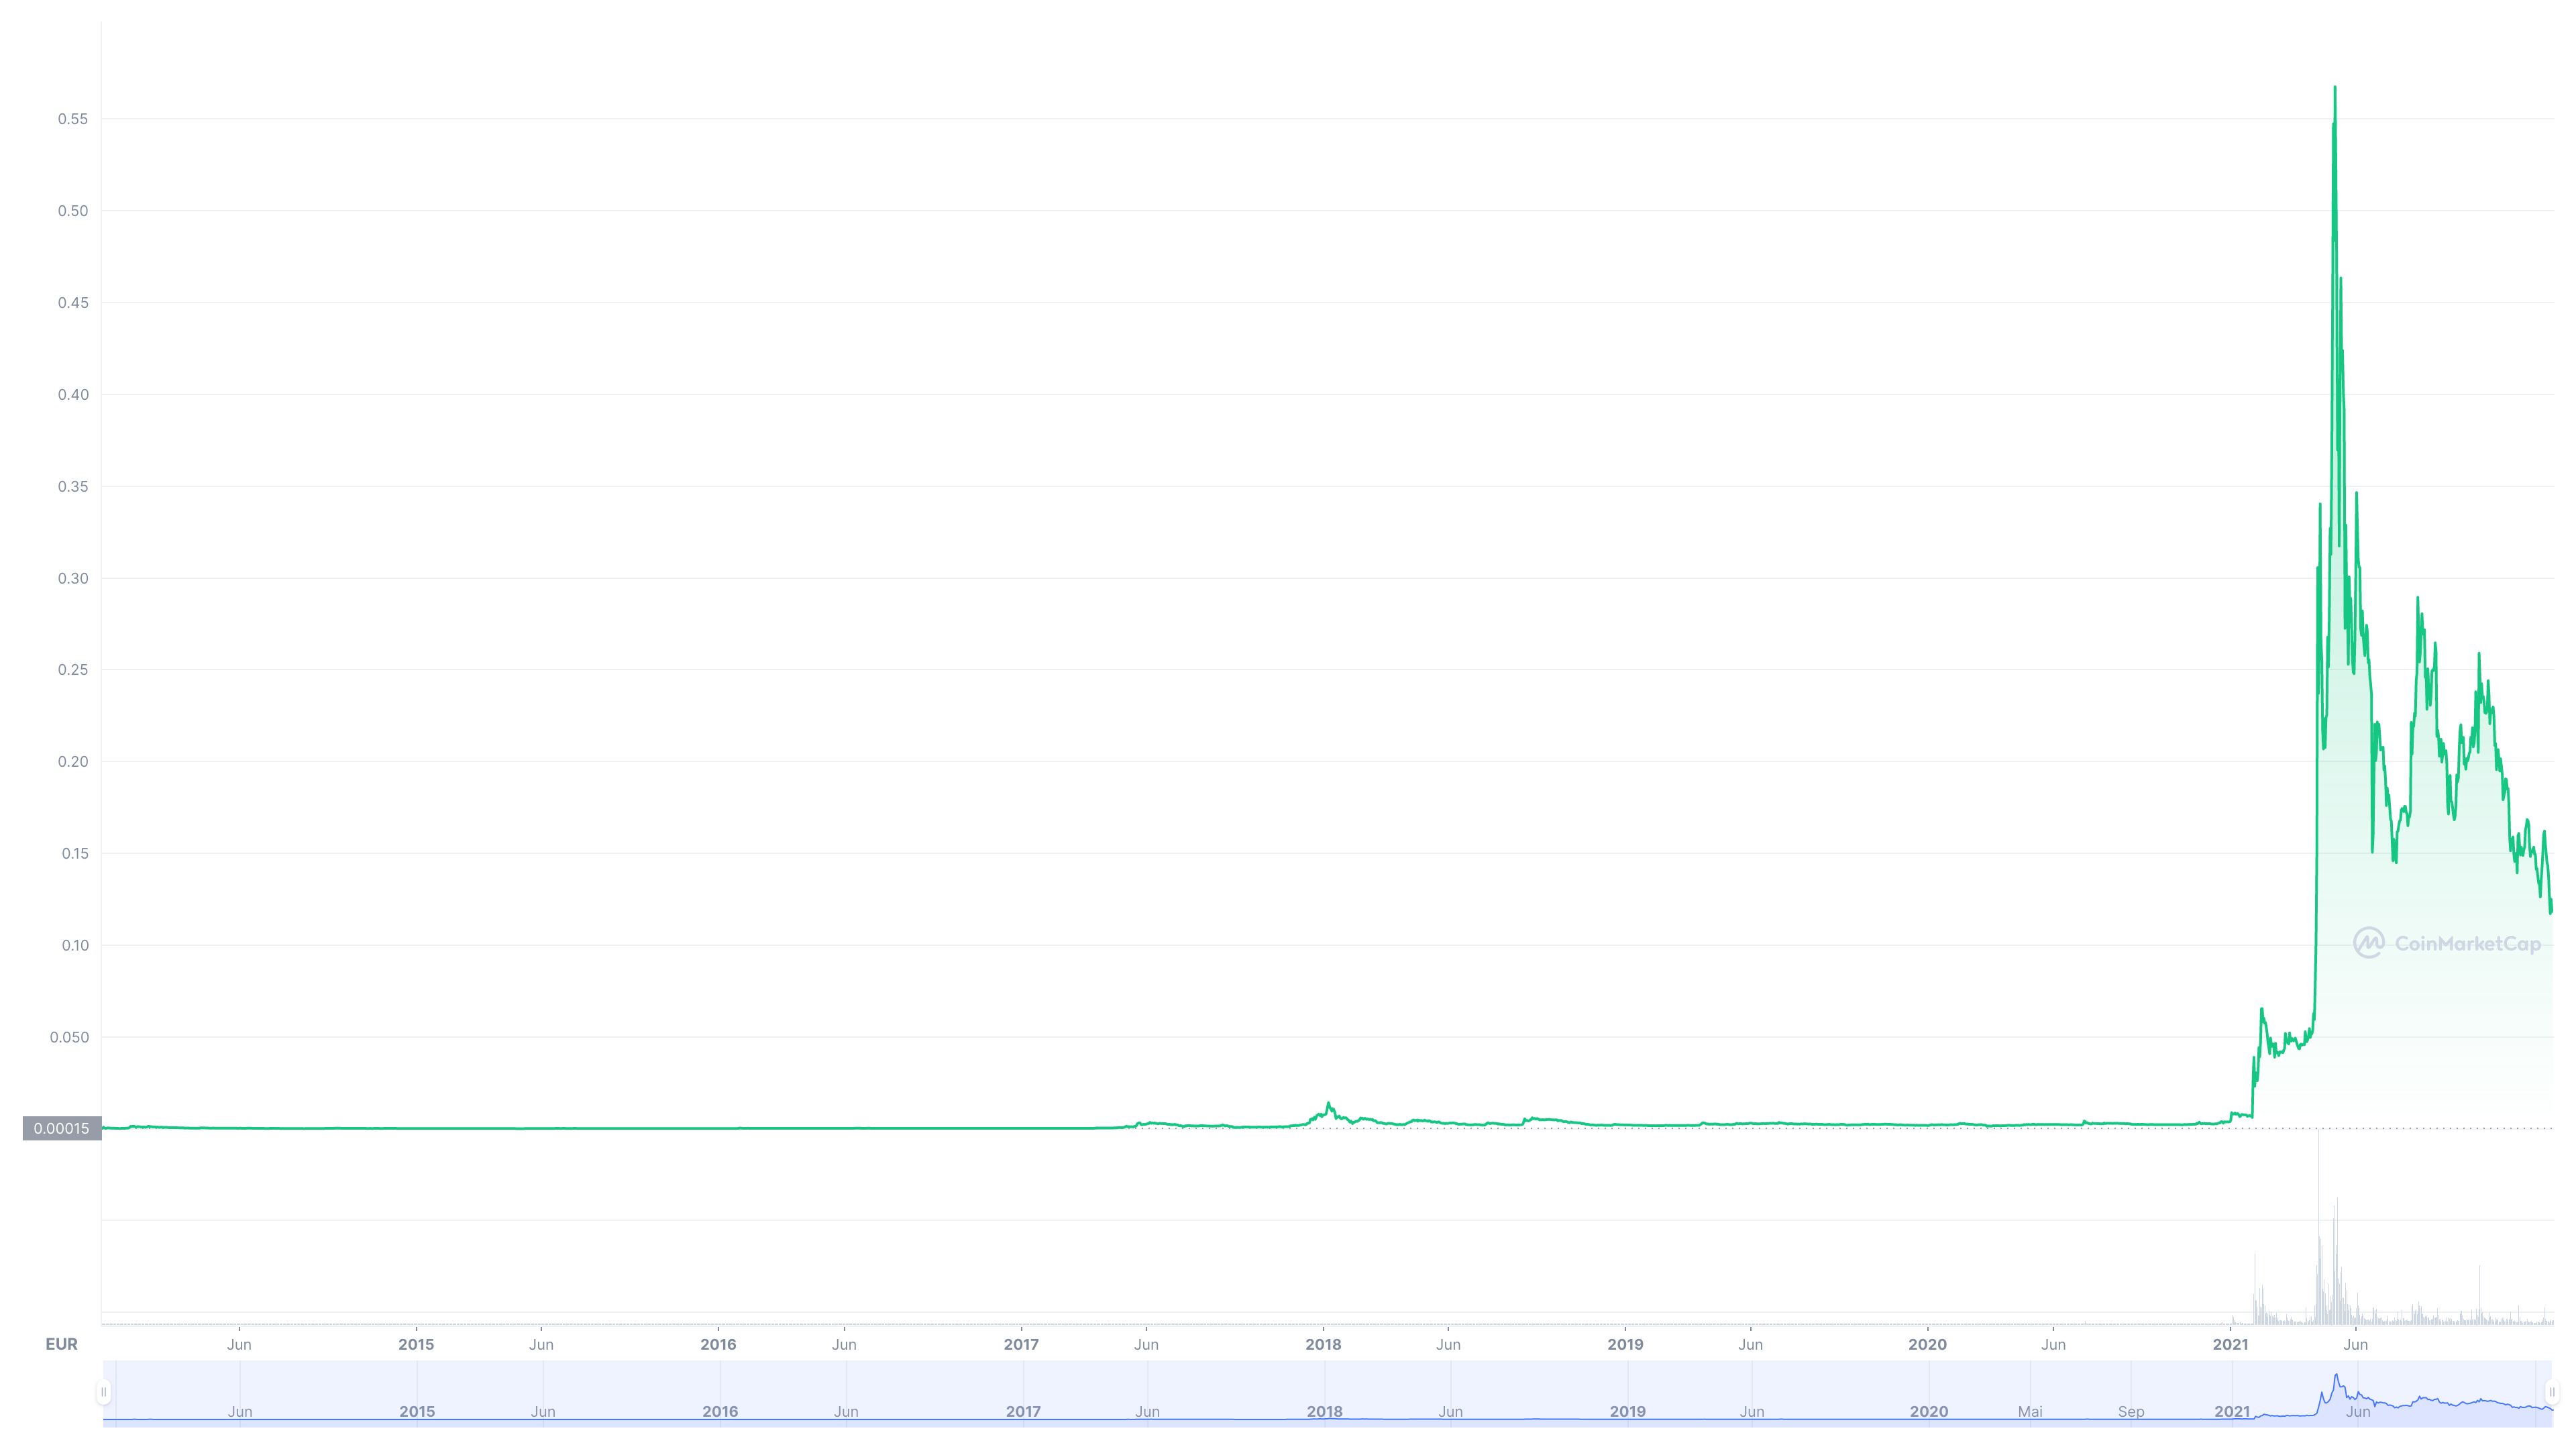
\includegraphics[width=0.8\textwidth]{graphics/Dogecoin.png}
    \caption{Historischer Wertekurs (Quelle: CoinMarketCap)}
\end{figure}

Am 8. April 2021 lag der Kurs bei 5 Cent, genau einen Monat später bei 52 Cent. Mit dieser mehr als 10-Fachung schaffte ''Dogecoin'' es bekanntlich sogar in die internationale Presse. Aber ist man stattdessen drei Monate früher eingestiegen, als am 6. Januar der Kurs noch bei $0.0085 \euro{}$ lag, hätte man sein Geld versechzigfachen können, wenn man schon anfang 2017 beim Preis von $0.000196 \euro{}$ eingestiegen wäre, hätte man sein Geld um den Faktor 2600 gesteigert. Das große Geld mit Cryptowährungen macht man also als ganz früher Einsteiger, lange bevor eine Währung populär ist und das Volumen so groß ist dass Preissteigerungen um 3 Großenordnungen ökonomisch unrealistisch sind.

Die entscheidene Frage ist jedoch, wie man drastische Kursänderungen bei völlig obskuren Coins vorhersagen kann. In unserer Ausarbeitung soll es darum gehen, ob Erwähnungen auf der Plattform Reddit ein brauchbarer Indikator sind.

Bei der Erhebung der Social Media Daten kam schnell das Problem auf, dass Reddits offizielle API auf 1000 Ergebnisse pro Suchanfrage limitiert ist. Jedoch existiert das inoffizielle ''Pushshift''-Archiv, das Suchen in einem präzisen Zeitrahmen ohne ein Limit für die Anzahl der Suchergebnisse ermöglicht. Aber auch da war mit einem Ratelimit von einer Anfrage pro Sekunde unsere geplante Auswertung von über 4000 Coins über einen Zeitraum von 4 Jahren nicht möglich. Also entschieden wir uns das komplette Pushshift-Archiv aller Kommentare auf Reddit herunterzuladen, dass in seinen 1.4 Terrabyte auf Academic Torrents (\url{https://academictorrents.com/details/90e7a746b1c24e45af0940b37cffcec7c96c8096}) als Peer-to-Peer-Download zur Verfügung steht. Wir beschränkten uns auf den Zeitraum vom 1. Januar 2017 bis zum 31. Dezember 2020 und ließen für jeden Tag die Anzahl der Erwähungen aller ausgewählten Cryptowährungen auswerten, was mehrere Tage Programmlaufzeit in Anspruch nahm. Um effizienter mit den Daten arbeiten zu können, sammelten wir die Erwähnungen in einer SQLite-Datenbank, bei dem der Schlüssel aus Datum und Coinname zusammengesetzt ist (bsp. ''2018-08-04-Bitcoin'').

Die Erhebung der Preisdaten im selben Zeitraum



























\end{document}